% !TEX root = /home/computer/ucsc/master-2/quarter-1/machine-learning/master.tex
\assignment{2}{Mon 18 Oct 2021 14:46}{Assignment 2}

\subsectionfont{\fontsize{10}{10}\selectfont}

\graphicspath{ {/home/computer/ucsc/master-2/quarter-1/machine-learning/assignment_02/figures/} }

\section{Problem 1}%
\begin{itemize}
  \item[ \textbf{a)} ] \textbf{How long would it take to test every possible
    hypothesis?}

    Instance space: 
    \[
      \{\text{Age status} \times \text{Residency} \times \text{Teeth} \times 
      \text{Sympathizes with}\times \text{Occupation}\}
    .\] 

    Number of instances: 
    \[
    3\times 2\times 2\times 3\times 4 = 144
    .\] 

    Then the number of possible hypothesis, and hence the number of nanoseconds
    testing a hypothesis would take 
    \[
      \boxed{2^{144} \quad \text{ns} }
    .\] 

  \item[ \textbf{b)} ] Conjunctive hypothesis space

    Number of hypothesis
    \[
      (3+1)\times (2+1)\times (2+1)\times (3+1)\times (4+1) = 720
    .\] 

    and hence it would take
    \[
      \boxed{720 \quad \text{ns}}
    .\] 

    to test every hypothesis in a conjunctive hypothesis space representation

  \item[ \textbf{c)} ]  \textbf{Conjunctive hypothesis space with internal
  disjunctions}

  Number of hypothesis
  \[
    |H| = 2^3-1\times 2^2-1\times 2^2-1\times 2^3-1\times 2^4-1 = 6615
  .\] 

  so it would take 
  \[
    \boxed{6615 \quad \text{ns}}
  .\] 

  to test every hypothesis

\end{itemize}


\section{Problem 2}%

The plane $3x_{1}+2x_{2}+4x_{3}=18$ has normal
\[
\vec{w} = \begin{pmatrix}
  3 \\
  2 \\
  4
\end{pmatrix}
.\] 

pointing in the direction of the positive class hypothesis.
\begin{figure}[H]
  \centering
  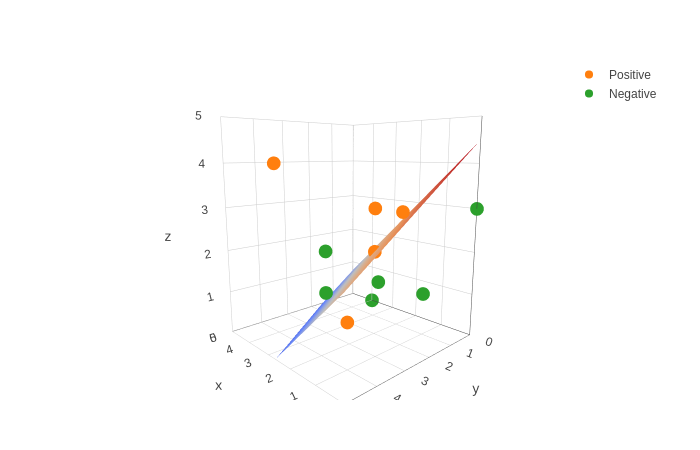
\includegraphics[width=0.8\linewidth]{newplot.png}
  \caption{Data}%
  \label{fig:Data}
\end{figure}

Calculating margin and loss yielded the following results

\begin{figure}[H]
  \centering
  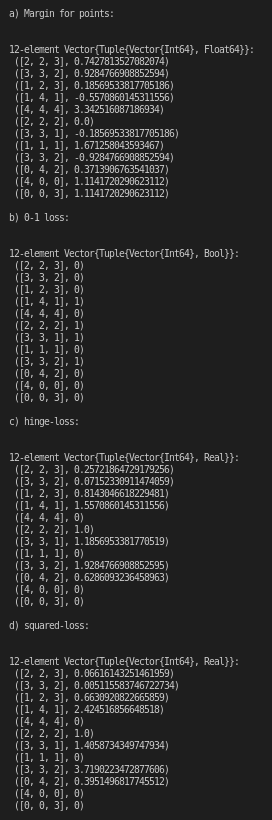
\includegraphics[width=0.5\linewidth]{prob2.png}
  \caption{prob2}%
  \label{fig:prob2}
\end{figure}

\section{Problem 3}%

Empirically estimating each class probability

\begin{figure}[H]
  \centering
  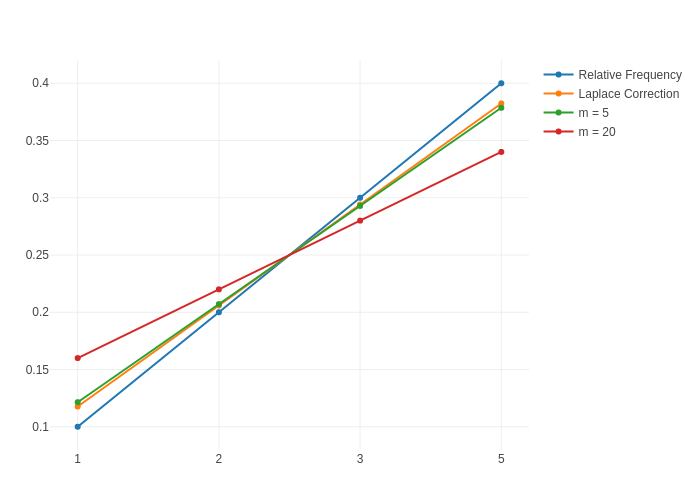
\includegraphics[width=0.8\linewidth]{prob3.png}
  \caption{prob3}%
  \label{fig:prob3}
\end{figure}

As we go from relative frequency to Laplace correction to m-estimates, we see
the estimates smooth out across each class. The m-estimate for $m=5$ is nearly
equal to Laplace correction due to the even distribution of pseudocounts at
$\frac{1}{4}$ being close to $\frac{1}{5}$ in which case it would be exactly
equal to the Laplace correction. So using a higher number $m = 20$ smooths
the data further.

\section{Problem 4}%

\begin{itemize}
\item[ \textbf{a)} ] \textbf{The number of conjunctive hypotheses} 

    Instance space: 
    \[
      \{\text{Budget} \times \text{Genre} \times \text{Famous actors} \times
      \text{Director}\}
    .\] 
    Number of hypothesis
    \[
      (3+1)\times (3+1)\times (2+1)\times (2+1) = \boxed{144}
    .\] 
  \item[ \textbf{b)} ] \textbf{Least general hypothesis for data $13$ and $16$} 

    \[
      \boxed{\text{Genre: Drama } \wedge \text{ Director: Great}}
    .\] 
  \item[ \textbf{c)} ] \textbf{Most general hypothesis for $13$, $16$, and $7$} 
    \[
      \boxed{\text{Genre: Drama}}
    .\] 
  \item[ \textbf{d)} ] \textbf{Least general hypothesis for data $10$, $11$,
    and $13$}
    \[
      \boxed{\text{Budget: Low} \wedge \text{Genre: Drama } \wedge \text{Famous
      actor: No} \wedge \text{ Director: Great}}
    .\] 
\end{itemize}

\section{Problem 5}%

Considering \textbf{Budget}, we break the data into those with \textbf{Low},
\textbf{Medium}, and \textbf{High} budgets. Then for each split we count the
number of positives $P$ and the number negatives $N$, then calculate the proportion
of positives $\hat{p} = \frac{P}{P+N}$ in each split and use the (entropy) impurity
measure for each
\[
  \text{Imp}(\hat{p}) = -\hat{p}log_2(\hat{p}) - (1-\hat{p})log_2(1-\hat{p})
.\] 

Multiply this by the number of data ($|D_{i}|$)in each split and then sum them up and
divide by the total number of data ($|D|$) in all splits
\[
  \sum_i \frac{|D_{i}|}{|D|}\text{Imp}(\hat{p})
.\] 
Then see how this value compares to Genre, Famous actors, and
Director, and pick the attribute (e.g. Budget) with the highest impurity measure.
The following figure is the result of forgetting to include the term
$\frac{|D_{i}|}{|D|}$ in the above sum. 

\begin{figure}[H]
  \centering
  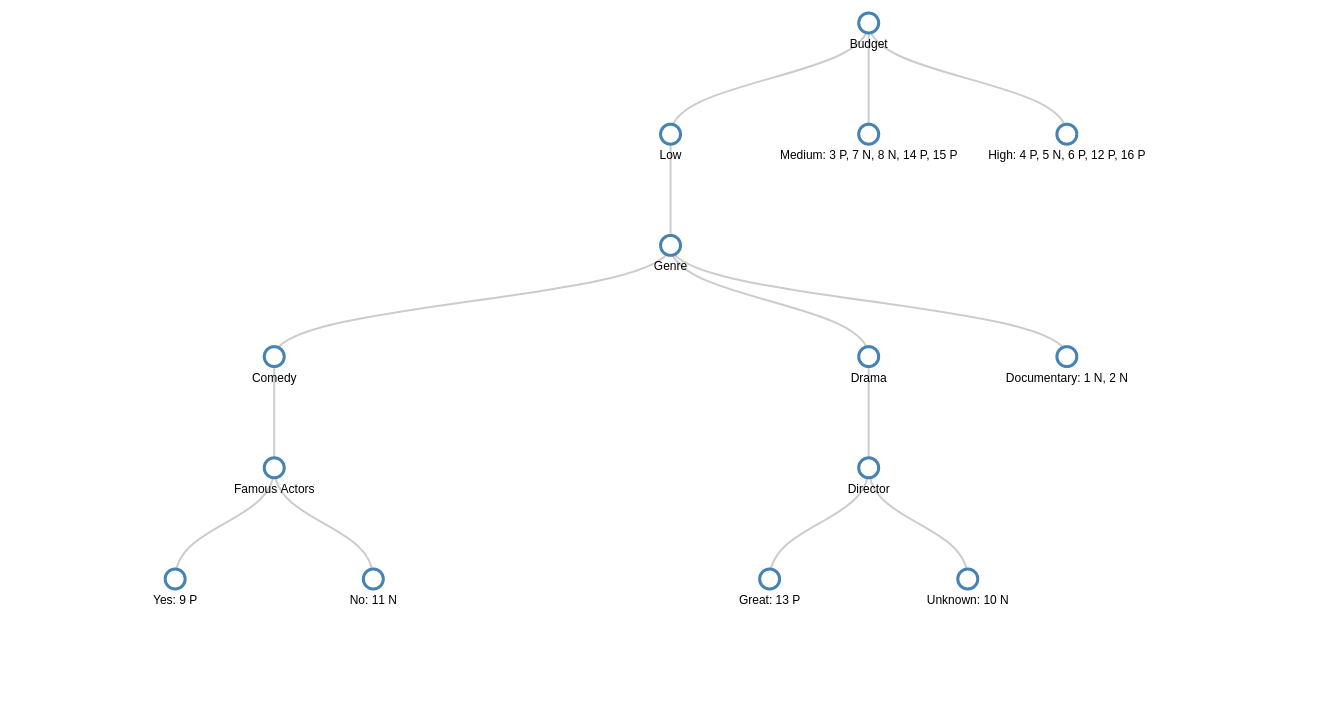
\includegraphics[width=0.8\linewidth]{labeled_tree.png}
  \caption{Labeled Training Tree}%
  \label{fig:labeled_tree}
\end{figure}

The following is the result of using this decision tree on the test data.

Testing data 1

\begin{figure}[H]
  \centering
  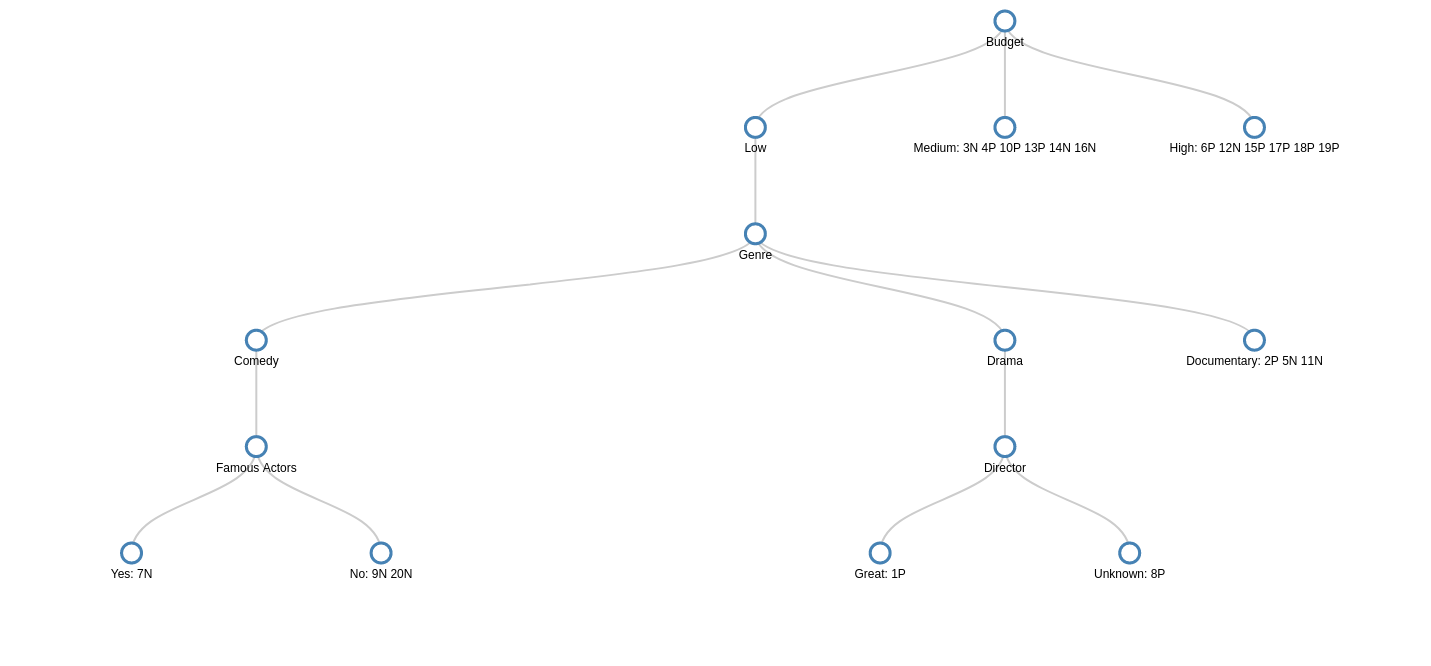
\includegraphics[width=0.8\linewidth]{tree1.png}
  \caption{Test1}%
  \label{fig:test1}
\end{figure}

Test data 2

\begin{figure}[H]
  \centering
  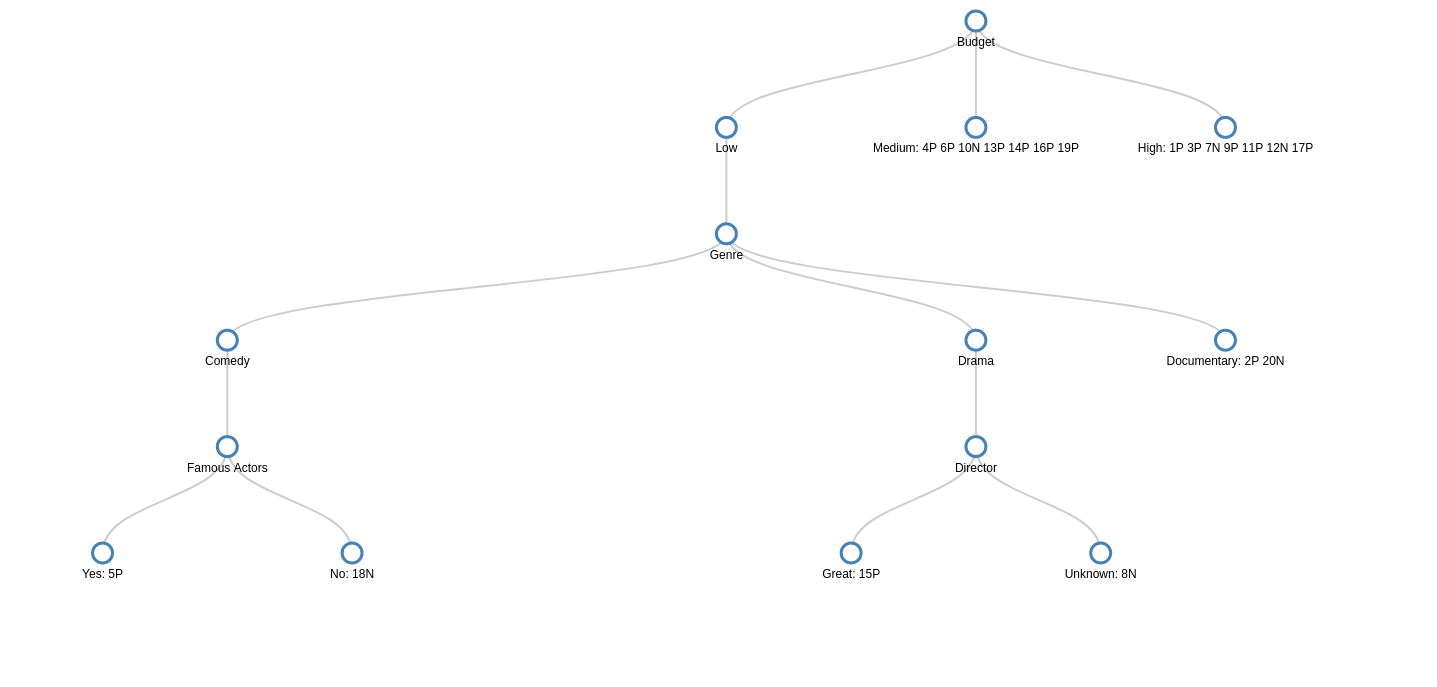
\includegraphics[width=0.8\linewidth]{test2.png}
  \caption{test2}%
  \label{fig:test2}
\end{figure}

Test data 3

\begin{figure}[H]
  \centering
  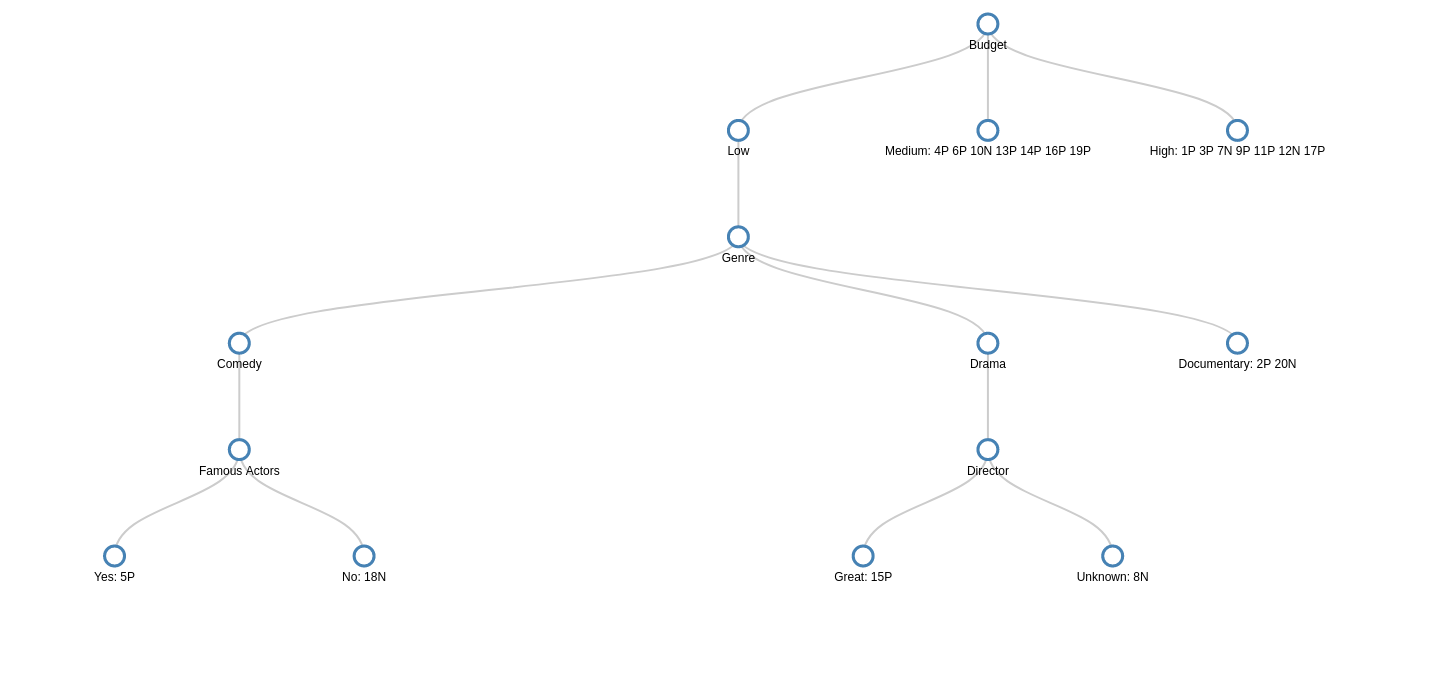
\includegraphics[width=0.8\linewidth]{test3.png}
  \caption{test3}%
  \label{fig:test3}
\end{figure}

\section{Problem 6}%

I wrote my code in julia, and I called it from the run.py file. I split the
training data into their respective classes $(0, 1, 2)$ and calculated the mean
along the $x$,  $y$, and $z$ components. This gave me the centroid of the each
class, and I used this to find the separating decision boundary.

\begin{figure}[H]
  \centering
  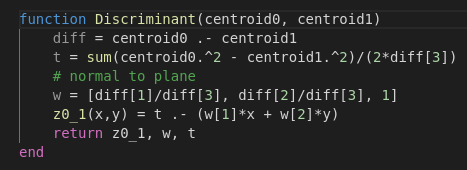
\includegraphics[width=0.8\linewidth]{discriminant.png}
  \caption{Discriminant}%
  \label{fig:discriminant}
\end{figure}

I then used the values $w, t$ to calculate the margin along decision boundary
between class 0 and class 1 in the training data. Then I checked which of these
the classifier mislabeled as class 0 or class 1 for the points that actually
belonged in class 2. 

\begin{figure}[H]
  \centering
  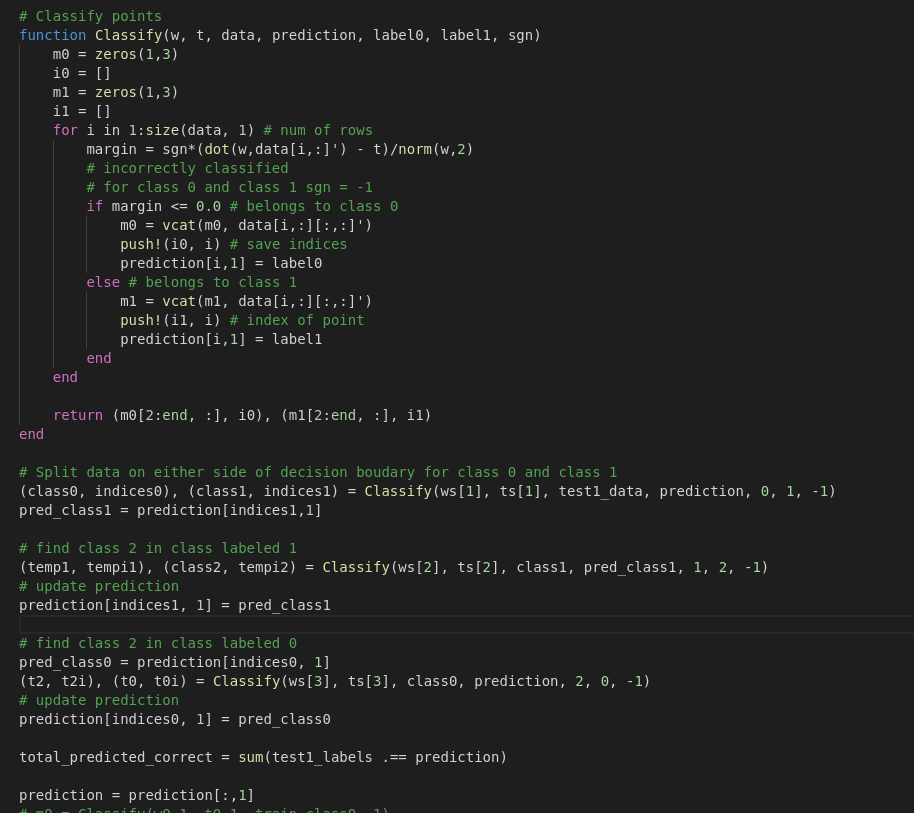
\includegraphics[width=0.8\linewidth]{classify.png}
  \caption{Classify}%
  \label{fig:classify}
\end{figure}
